% =============================================================================
% File:  MATLAB1.tex -- 
% Author(s): Valentin Plugaru (valentin.plugaru@uni.lu)
% Time-stamp: <Tue 2015-06-16 09:22 svarrette>
% 
% Copyright (c) 2015 Valentin Plugaru<Valentin.Plugaru@uni.lu>
% 
% For more information:
% - LaTeX: http://www.latex-project.org/
% - Beamer: https://bitbucket.org/rivanvx/beamer/
% - LaTeX symbol list:
% http://www.ctan.org/tex-archive/info/symbols/comprehensive/symbols-a4.pdf
% =============================================================================

\documentclass{beamer}
% \documentclass[draft]{beamer}
\usepackage{_style}
\newcommand{\cmdlinegaia}[1]{\promptline{(gaia)}{#1}}
\newcommand{\cmdlinechaos}[1]{\promptline{(chaos)}{#1}}
\newcommand{\cmdlinefrontend}[1]{\promptline{(frontend)}{#1}}
\newcommand{\cmdlinenode}[1]{\promptline{(node)}{#1}}
\newcommand{\cmdlinecomment}[1]{\hfill{\tiny \textcolor{red}{\textit{\# #1}}}}
\newcommand{\ULHPC}{\href{http://hpc.uni.lu}{UL HPC Platform}\xspace}


% The key part to use my theme -- if you precise nothing, the image that
% illustrate the slides is assumed to be images/slides_image.jpg
\usetheme[image=images/logo_hpc-shool2015.pdf]{Falkor}

% Not integrated in my theme as not everybody wants that
\AtBeginSection[]
{
  \frame{
    \frametitle{Summary}
    {\scriptsize\tableofcontents[currentsection]}
  }
}

\graphicspath{{images/}} % Add this directory to the searched paths for graphics


%%%%%%%%%% Header %%%%%%%%%%%%
\title{MATLAB on UL HPC}
\subtitle{Interactive \& passive jobs, sequential and XCS execution}

\author{Valentin Plugaru}
\institute[UL HPC, PCOG Research unit]{
  \href{http://hpc.uni.lu}{UL HPC} Management Team,\\
  Parallel Computing and Optimization Group (\href{http://pcog.uni.lu}{PCOG}),
  University of Luxembourg (\href{http://www.uni.lu}{UL}), Luxembourg
}

% Mandatory to **declare** a logo to be placed on the bottom right -- normally the
% university logo. ADAPT ACCORDINGLY:
\pgfdeclareimage[height=0.8cm]{logo}{images/logo_UL.pdf}

\date{}

%%%%%%%%%%%%% Body %%%%%%%%%%%%%%%
\begin{document}

\begin{frame}
  \vspace{2.5em}
  \titlepage
\end{frame}

\begin{frame}
  \begin{center}
      \textbf{Latest versions available on
        \href{https://github.com/ULHPC/}{Github}}:
      \vfill
      \begin{description}
        \item[UL HPC tutorials:] \hfill
          \myurl{https://github.com/ULHPC/tutorials}
        \item[UL HPC School:] \hfill
          \myurl{https://hpc.uni.lu/hpc-school}
        \item[This tutorial's sources:] \hfill
          \myurl{https://github.com/ULHPC/tutorials/tree/devel/advanced/MATLAB1}
      \end{description}
  \end{center}
\end{frame}

% ......
\frame{
  \frametitle{Summary}
  {\scriptsize
    \tableofcontents
  }
}

\section{Pre-requisites}

% .......
\begin{frame}[fragile]
\frametitle{Tutorial files}
  Sample MATLAB scripts used in the tutorial\\
  \begin{itemize}
   \item download only the scripts: \\
  \begin{cmdline}
    \cmdlinefrontend{mkdir \$HOME/matlab-tutorial} \\
    \cmdlinefrontend{cd \$HOME/matlab-tutorial} \\
    \cmdlinefrontend{wget \myurl{https://raw.github.com/ULHPC/tutorials/devel/advanced/MATLAB1/code/example1.m}} \\
    \cmdlinefrontend{wget \myurl{https://raw.github.com/ULHPC/tutorials/devel/advanced/MATLAB1/code/example2.m}} \\
    \cmdlinefrontend{wget \myurl{https://raw.github.com/ULHPC/tutorials/devel/advanced/MATLAB1/code/yahoo\_finance\_data.m}} \\
  \end{cmdline}
  \item \textit{or} download the full repository and link to the MATLAB tutorial: \\
  \begin{cmdline}
    \cmdlinefrontend{git clone \myurl{https://github.com/ULHPC/tutorials.git}} \\
    \cmdlinefrontend{ln -s tutorials/advanced/MATLAB1/ \$HOME/matlab-tutorial} \\
  \end{cmdline}  
  \end{itemize}

\end{frame}

\begin{frame}[fragile]
\frametitle{X Window System}
  In order to see locally the MATLAB graphical interface, \\
  a package providing the X Window System is required:
  \begin{itemize}
    \item on OS X: \textbf{XQuartz} \hfill\myurl{http://xquartz.macosforge.org/landing/}
    \item on Windows: \textbf{VcXsrv} \hfill\myurl{http://sourceforge.net/projects/vcxsrv/}
  \end{itemize}
  \hfill \\ \hfill \\ %\hfill \\
  
  Now you will be able to connect with X11 forwarding enabled:
  \begin{itemize}
    \item on Linux \& OS X: \\
    \begin{cmdline}
       \cmdlineentry{ssh access-gaia.uni.lu} \textbf{-X}
    \end{cmdline}
    \item on Windows, with Putty \\
     Connection $\rightarrow$ SSH $\rightarrow$ X11 $\rightarrow$ \textbf{Enable X11 forwarding}
  \end{itemize}  
\end{frame}

% ===============================================
\section{Objectives}

% ............
\begin{frame}
  \frametitle{Objectives of this PS}

  Better understand the usage of MATLAB on the \ULHPC
 
  \begin{exampleblock}{}
    \begin{itemize}
      \item running in interactive mode
      \begin{itemize}
        \item with either the full graphical or the text-mode interface
        \item using the XCS portal (\href{https://xcs.uni.lux}{xcs.uni.lux})
      \end{itemize}
     \end{itemize}
     \vspace{-1.5ex}
   \end{exampleblock}
   \pause
   \begin{exampleblock}{}
    \begin{itemize}
     \item running in passive mode
      \begin{itemize}
       \item several ways of submitting MATLAB jobs
      \end{itemize}
     \end{itemize}
    \vspace{-1.5ex}
    \end{exampleblock}
   \pause
   \begin{exampleblock}{}
    \begin{itemize}
     \item checking available toolboxes \& licenses status
    \end{itemize}
   \vspace{-1.5ex}
   \end{exampleblock}
   \pause
   \begin{exampleblock}{}
    \begin{itemize}
     \item using script (.m) files
    \end{itemize}
   \vspace{-1.5ex}
   \end{exampleblock}
   \pause
   \begin{exampleblock}{}
    \begin{itemize}
     \item plotting data, saving the plots to file
% 	\item taking advantage of some parallelization capabilities
%           \begin{itemize}
%               \item use of \textbf{parfor}
%               \item use of GPU-enabled functions
%           \end{itemize}
    \end{itemize}
    \vspace{-1.5ex}
   \end{exampleblock}
\end{frame}

\section{Example 1}

% .......
\frame{
  \frametitle{Scripts and plots}
  \textbf{example1.m}: non-interactive script that shows:
\begin{itemize}
 \item the use of a stopwatch timer
 \item how to use an external function (financial data retrieval)
 \item how to use different plotting methods
 \item how to export the plots in different graphic formats
\end{itemize} 
 \includegraphics[width=0.45\linewidth,keepaspectratio]{plots/example1-2dplot.eps}
 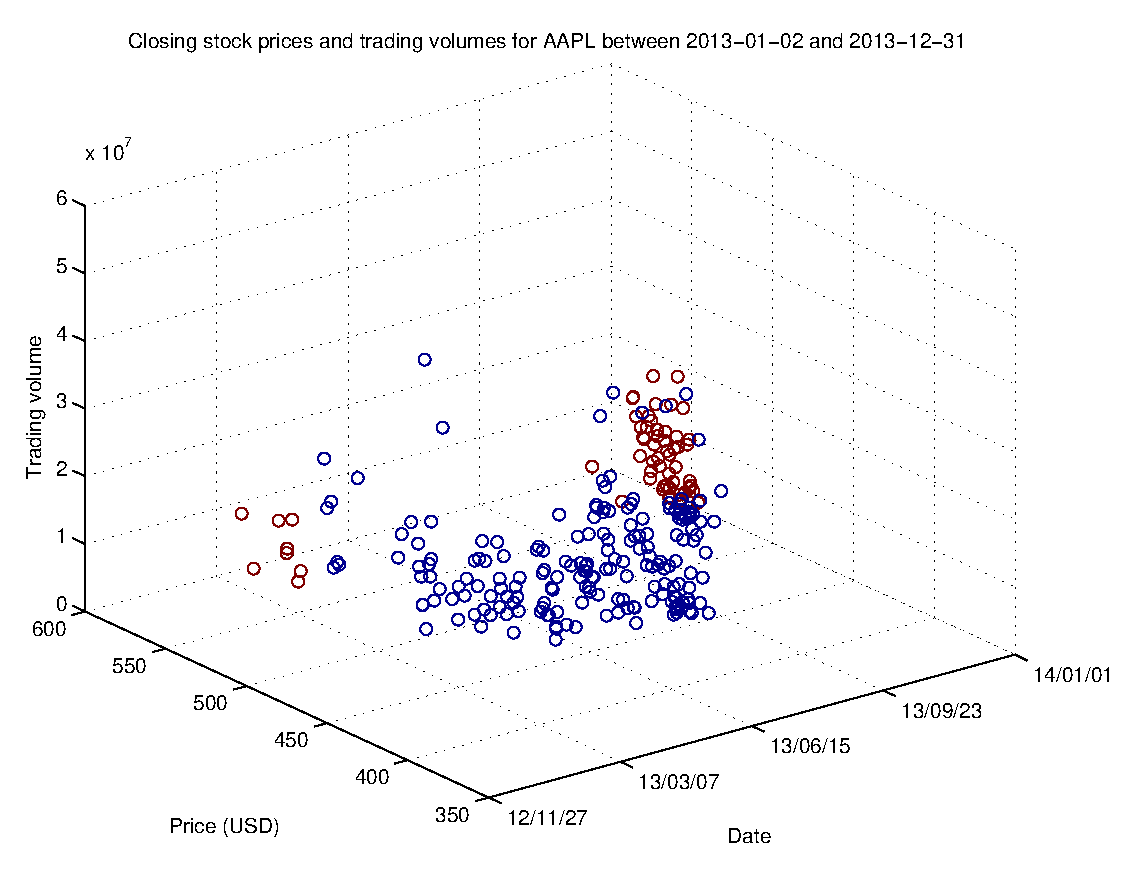
\includegraphics[width=0.45\linewidth,keepaspectratio]{plots/example1-scatter.eps}  
}

\section{Example 2}

% .......
\frame{
  \frametitle{Parallelization}
  \textbf{example2.m}: non-interactive script that shows:
  \begin{itemize}
   \item the serial execution of time consuming operations
   \pause
   \item Revisited in MATLAB2 tutorial:
   \begin{itemize}
    \item the parallel execution and relative speedup vs serial execution
    \item setting the \# of parallel threads through environment variables
    \item GPU-based parallel execution
    \end{itemize}
  \end{itemize}
  \centering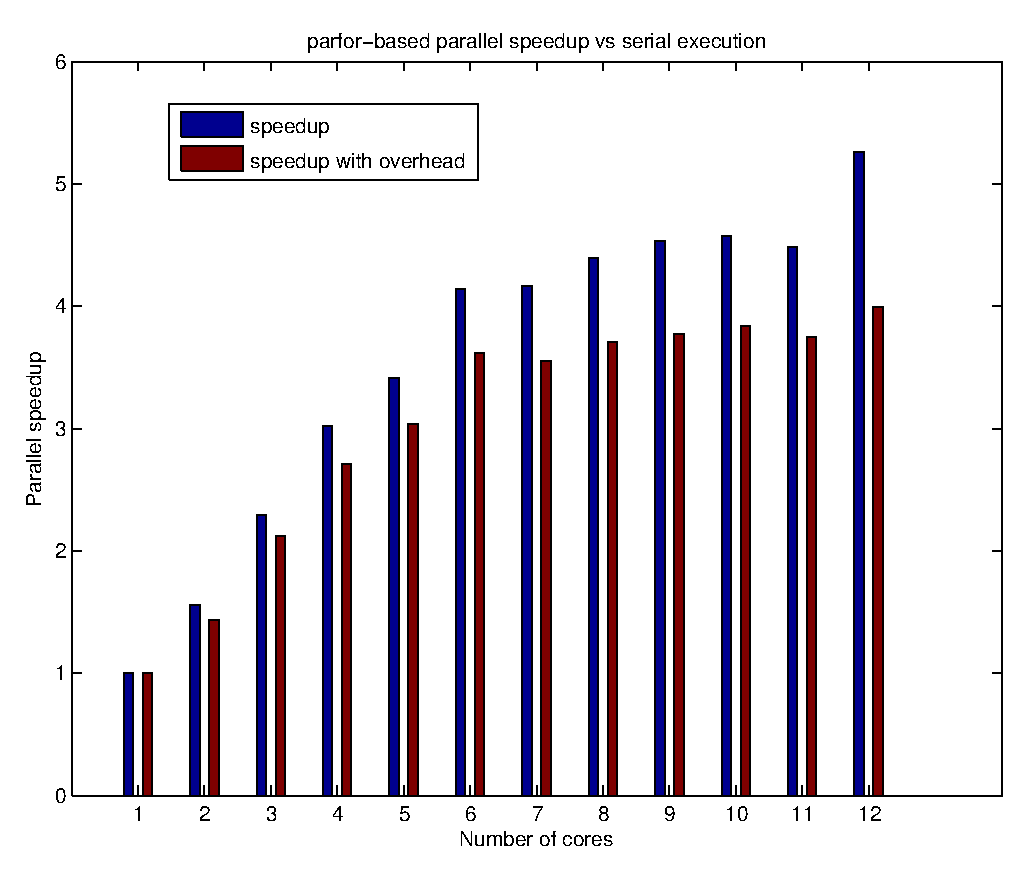
\includegraphics[width=0.45\linewidth,keepaspectratio]{plots/parfor-speedup.eps}
}

\section{Practical session}

% .......
\begin{frame}
  \frametitle{Exercises}
    \begin{itemize}
      \item Read and understand the MATLAB tutorial \myurl{https://github.com/ULHPC/tutorials/tree/devel/advanced/MATLAB1} \\
      $ \hookrightarrow $ \scriptsize{all provided scripts are fully commented}
      \item Run all the examples \\
      $ \hookrightarrow $ launching interactive/passive mode MATLAB \\
      $ \hookrightarrow $ plotting script \\
      $ \hookrightarrow $ parallel execution script \\
%       \item Plot the speedup graph shown at \href{https://github.com/ULHPC/tutorials/tree/devel/advanced/MATLAB1\#useful-references}{tutorial's end}
    \end{itemize}
\end{frame}

\begin{frame}
  \frametitle{Useful links}
  \begin{itemize}
   \item Parallel Computing Toolbox \hfill\myurl{http://www.mathworks.nl/help/distcomp/index.html}
   \item Parallel for-Loops (parfor) \hfill\myurl{http://www.mathworks.nl/help/distcomp/getting-started-with-parfor.html}
   \item GPU Computing \hfill\myurl{http://www.mathworks.nl/discovery/matlab-gpu.html}
  \end{itemize}
\end{frame}


\section{Conclusion}
% ............
\begin{frame}
  \frametitle{What we've seen so far}
   
   \begin{itemize}
     \item MATLAB execution modes on the \ULHPC
     \item Checking for available toolboxes and licenses
     \item Plotting
   \end{itemize}

    \begin{block}{Perspectives}
      \begin{itemize}
        \item Personalize the UL HPC launchers with the MATLAB commands
        \item Check the second example M-file for insight into basic parallel execution
        \item Parallelize your own tasks using parfor/GPU-enabled instructions
      \end{itemize}
    \end{block}

\end{frame}


% ======================== END =========================
\section*{Thank you for your attention...}
\frame{
  \frametitle{Questions?}
  % ~~~~~~~~~~~~~~
  \begin{columns}
    \column{0.5\textwidth}
    % \emph{Contact}\\
    {\tiny
      \emph{Valentin Plugaru}\\
      ~~~~ \textit{Mail:} \href{mailto:valentin.plugaru@uni.lu}{valentin.plugaru@uni.lu}\\
      ~~~~ Office E-005\\
      ~~~~ Campus Kirchberg\\
      ~~~~ 6, rue Coudenhove-Kalergi\\
      ~~~~ L-1359 Luxembourg\\[1em]
 
      \emph{UL HPC Management Team}\\
      ~~~~ \textit{mail:} \href{mailto:hpc-sysadmins@uni.lu}{hpc-sysadmins@uni.lu}\\
      


    }
    \column{0.5\textwidth}
    % \scalebox{8}{\emph{?}}
    
\includegraphics[width=1.5in]{question.jpg}
  \end{columns}
  % Below is the table of content over 2 columns
  \vfill
%  \begin{multicols}{2}
    {\tiny \tableofcontents}
%  \end{multicols}

}

\newcounter{finalframe}
\setcounter{finalframe}{\value{framenumber}}

% %.......
% \frame{
%   \frametitle{}
%   \vfill
%   \centering \LARGE Appendix\footnote{notice the slide number below...}
%   \vfill
% }

\setcounter{framenumber}{\value{finalframe}}

\end{document}

% ~~~~~~~~~~~~~~~~~~~~~~~~~~~~~~~~~~~~~~~~~~~~~~~~~~~~~~~~~~~~~~~~
% eof
% 
% Local Variables:
% mode: latex
% mode: flyspell
% mode: visual-line
% TeX-master: "MATLAB1.tex"
% End:
